\section{Methodology, Results, and Analysis}\label{sec:results}

\subsection{Methodology}

\subsubsection{Evaluation Metric}

The primary evaluation metric we used is strategy accuracy. The fraction of race-driver combinations where the system's predicted 
first pit lap is within $\pm 5$ laps of the nearest actual pit lap. Formally, for the set of evaluated race-driver pairs $R$, 
with predicted first pit $\hat{p}_r$ and nearest actual pit $p_r^*$:
\begin{equation}
\text{StratAcc} = \frac{1}{|R|}\sum_{r \in R}\mathbb{1}\!\left[\,|\hat{p}_r - p_r^*| \leq 5\,\right]
\end{equation}
The $\pm 5$ lap tolerance reflects the real variance in F1 team strategy decisions since the same race scenario is often handled 5--10 
laps differently by different teams, making strict lap accuracy an unreasonably tight criterion~\cite{heilmeier2020}.

MAE on the held-out 2024 lap time sequences is reported as a secondary metric:
\begin{equation}
\text{MAE} = \frac{1}{N}\sum_{i=1}^{N}|\hat{y}_i - y_i|
\end{equation}
but is shown across multiple experiments to be a poor proxy for strategy accuracy (see Section~\ref{sec:analysis}).

Two no-parameter baselines are used. The \textit{moving average baseline} (used for absolute lap-time targets) predicts each lap's time as the mean of the 10 preceding laps:
\begin{equation}
\hat{y}_i^\text{base} = \frac{1}{10}\sum_{k=1}^{10} t_{i-k}.
\end{equation}
The \textit{mean-delta baseline} (used for delta targets, including the compound-specific results in Table~\ref{tab:compound}) predicts the next lap-to-lap change as the mean of the 9 lap-to-lap deltas observed within the input window:
\begin{equation}
\widehat{\Delta y}_i^\text{base} = \frac{1}{9}\sum_{k=1}^{9} (t_{i-k} - t_{i-k-1}).
\end{equation}
All MAE improvements are reported relative to whichever baseline matches the model's training target.

\subsubsection{Test Set}

The 2024 Formula 1 season (24 rounds) is held out entirely for strategy evaluation. Models see no 2024 data during training or 
hyperparameter tuning. The final expanded evaluation covers 6 drivers---VER (Verstappen, Red Bull), NOR (Norris, McLaren), 
LEC (Leclerc, Ferrari), SAI (Sainz, Ferrari), HAM (Hamilton, Mercedes), RUS (Russell, Mercedes)---across all 24 rounds, 
producing up to 144 race-driver combinations. Combinations where a driver retired or did not make a pit stop under green-flag 
conditions are automatically skipped, yielding 122 valid evaluations.

\subsection{Results}

\subsubsection{Architecture Comparison}

Table~\ref{tab:architectures} summarizes all model configurations evaluated across three data versions. The GRU architecture (hidden=64, layers=2, dropout=0.2) is the consistent winner across all data configurations, and is selected as the base for all subsequent strategy-level experiments.

\begin{table}[ht]
\centering
\caption{MAE Results Across Architectures and Data Versions}
\label{tab:architectures}
\begin{tabular}{llrrr}
\toprule
Architecture & Config & MAE & vs.\ Baseline & Stopped Epoch \\
\midrule
\multicolumn{5}{l}{\textit{Run 1 --- 2023 only ($\sim$14k sequences), baseline MAE = 0.0957}} \\
LSTM & hidden=64, dropout=0.2 & 0.0914 & +4.5\% & 34 \\
LSTM & hidden=128, dropout=0.2 & 0.1158 & $-$20.9\% & 32 \\
LSTM & hidden=64, layers=3, dropout=0.3 & 0.1016 & $-$6.2\% & 30 \\
LSTM & hidden=64, dropout=0.4 & 0.0656 & +31.5\% & 31 \\
\textbf{GRU} & \textbf{hidden=64, dropout=0.2} & \textbf{0.0575} & \textbf{+39.9\%} & \textbf{21} \\
\midrule
\multicolumn{5}{l}{\textit{Run 2 --- 2022+2023 (28k sequences), baseline MAE = 0.0957}} \\
LSTM & hidden=64, dropout=0.2 & 0.1044 & $-$9.0\% & 32 \\
LSTM & hidden=128, dropout=0.2 & 0.1092 & $-$14.1\% & 33 \\
LSTM & hidden=64, layers=3, dropout=0.3 & 0.0819 & +14.5\% & 31 \\
LSTM & hidden=64, dropout=0.4 & 0.0698 & +27.1\% & 33 \\
LSTM + Attention & hidden=64, dropout=0.2 & 0.1173 & $-$22.5\% & 28 \\
\textbf{GRU} & \textbf{hidden=64, dropout=0.2} & \textbf{0.0589} & \textbf{+38.5\%} & \textbf{24} \\
\midrule
\multicolumn{5}{l}{\textit{Run 3 --- 2022+2023, green-flag filter only, baseline MAE = 0.0605}} \\
LSTM & hidden=64, dropout=0.2 & 0.1116 & $-$84.4\% & --- \\
LSTM & hidden=64, dropout=0.4 & 0.0464 & +23.3\% & --- \\
\textbf{GRU} & \textbf{hidden=64, dropout=0.2} & \textbf{0.0363} & \textbf{+40.0\%} & \textbf{---} \\
\bottomrule
\end{tabular}
\end{table}

Figure~\ref{fig:training_curves} shows training and validation loss curves for the best LSTM and GRU configurations from Run 1. 
The GRU converges in 21 epochs versus 30+ for LSTM, and its train to validation gap is visibly narrower, consistent with lower overfitting risk at 
this dataset size. Figure~\ref{fig:mae_comparison} shows the test MAE for the three main Run 1 configurations: the GRU achieves a 40\% reduction 
over the moving average baseline while the default LSTM slightly exceeds baseline MAE.

\begin{figure}[htbp]
\centering
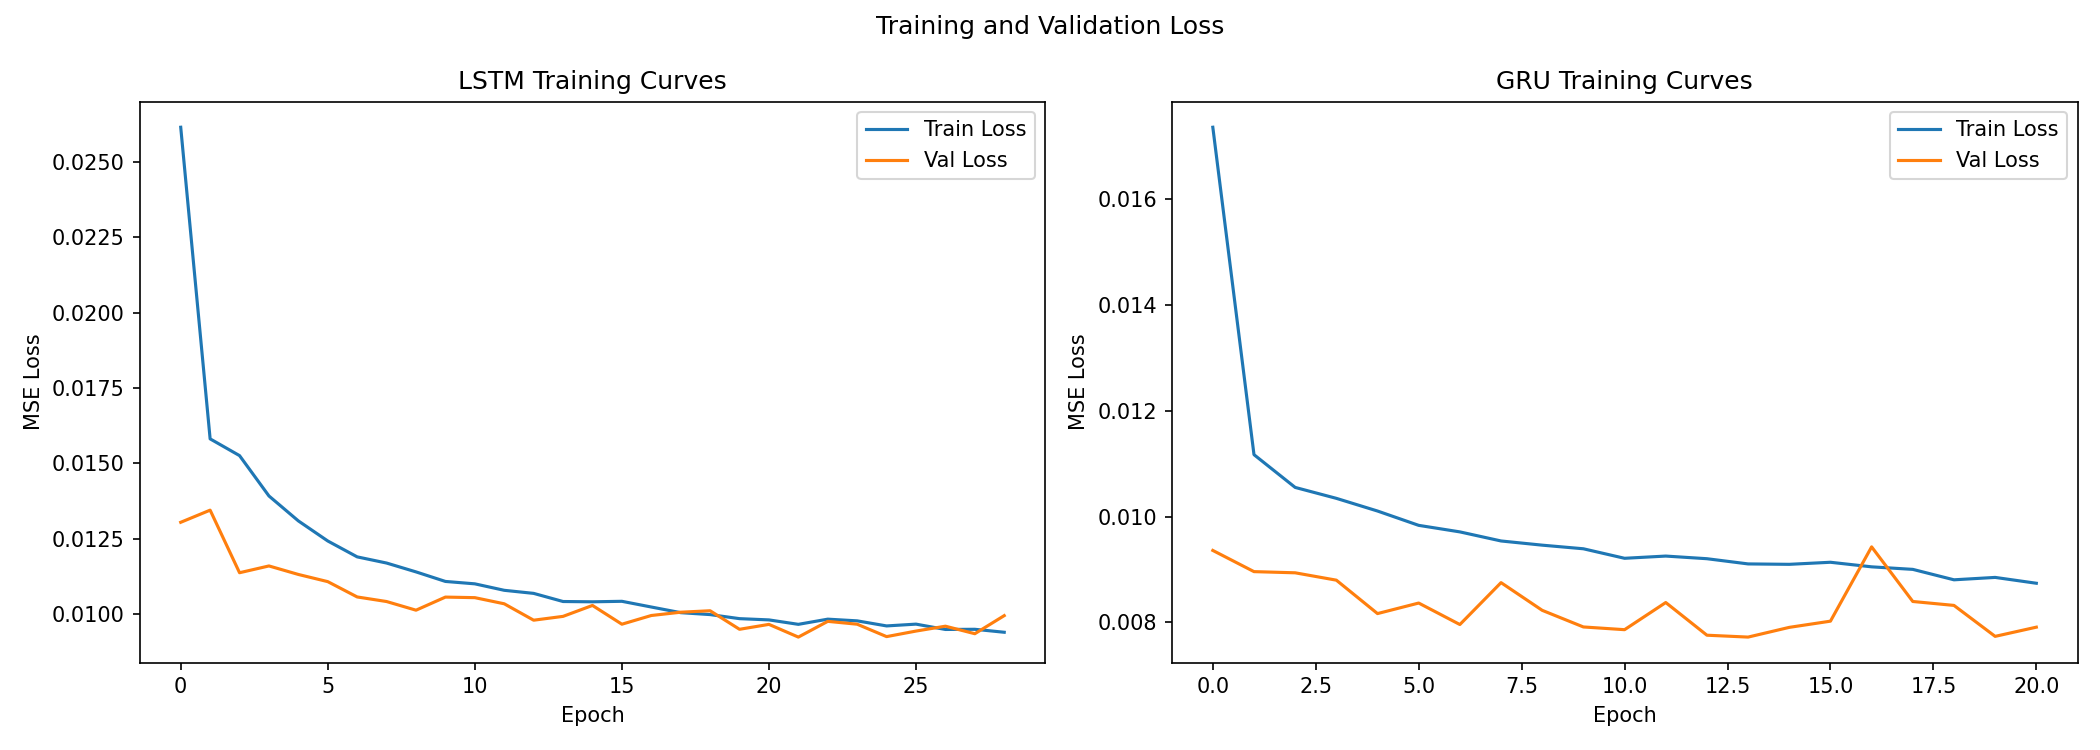
\includegraphics[width=\textwidth]{../results/training_curves.png}
\caption{Training and validation loss curves for the best LSTM (left) and GRU (right) configurations (Run 1). The GRU converges faster and shows a 
tighter train--validation gap, indicating less overfitting.}
\label{fig:training_curves}
\end{figure}

\begin{figure}[htbp]
\centering
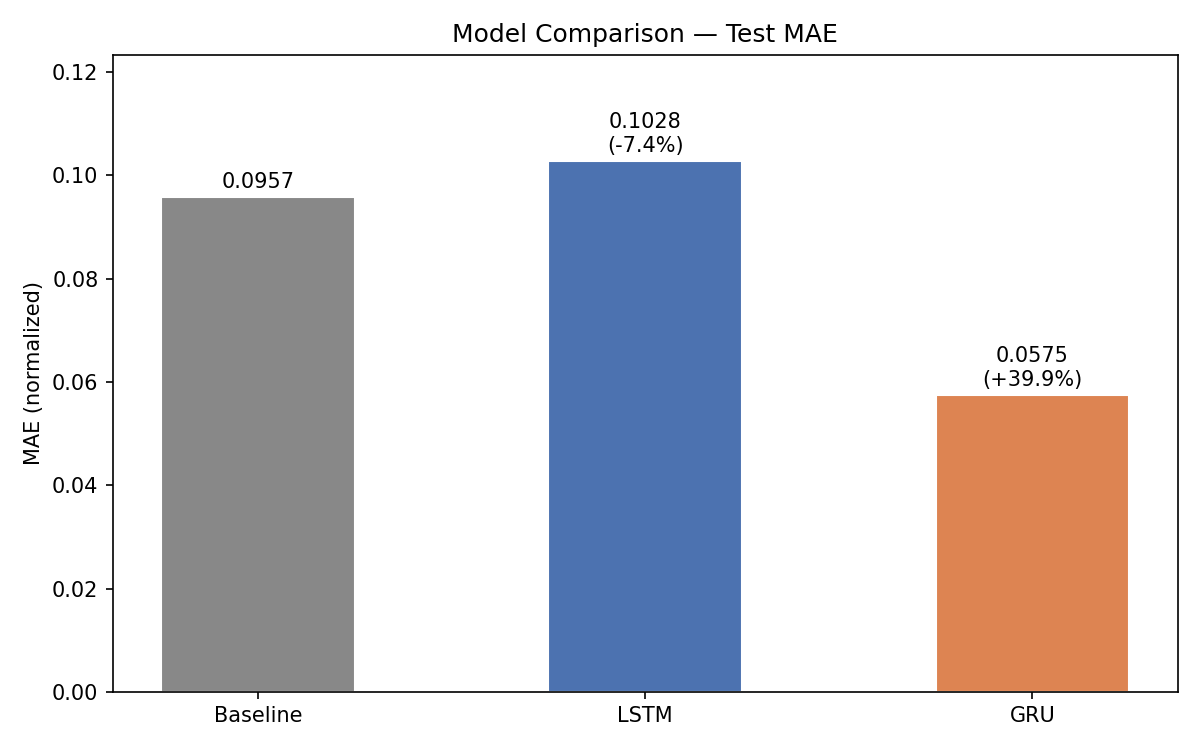
\includegraphics[width=0.65\textwidth]{../results/mae_comparison.png}
\caption{Test MAE for the baseline, best LSTM, and GRU on Run 1 (2023 data, 14k sequences). The GRU achieves a 39.9\% improvement over the moving 
average baseline; the default LSTM slightly underperforms it.}
\label{fig:mae_comparison}
\end{figure}

\subsubsection{Strategy Accuracy Progression}

Table~\ref{tab:strategy} traces strategy accuracy across all five phases of strategy-level development. The largest single jump is Phase 2 
(+26.2 percentage points), driven by splitting training by tire compound. Phase 3 and Phase 4 both regressed and were reverted; the final system
 uses the Phase 2 compound-specific configuration evaluated over 122 race-driver combinations.

\begin{table}[ht]
\centering
\caption{Strategy Accuracy Across All Phases}
\label{tab:strategy}
\begin{tabular}{lllr}
\toprule
Phase & Key Change & Evaluations & Accuracy \\
\midrule
Baseline (single-stop, shared GRU) & --- & 42 & 31.0\% \\
Phase 1: Multi-stop simulation & Brute-force 2-stop search & 42 & 35.7\% \\
Phase 2: Compound-specific GRUs & Separate model per compound & 42 & 61.9\% \\
Phase 3: Min first-pit constraint & Hard minimum lap threshold & 42 & 59.5\% (reverted) \\
Phase 4: Longer sequence (seq=15) & Window length 10$\to$15 laps & 42 & 50.0\% (reverted) \\
\textbf{Phase 5: 6-driver eval} & \textbf{Expanded to 122 evaluations} & \textbf{122} & \textbf{52.5\%} \\
\bottomrule
\end{tabular}
\end{table}

\subsubsection{Compound-Specific Model Results (Phase 2)}

Separate GRU models are trained on sequences filtered by the compound active at each timestep. Table~\ref{tab:compound} shows training results 
for the three compound-specific models. The HARD model benefits most from the compound split (14.1\% lower MAE than the mean-delta baseline), likely because hard-compound
stints are longer and the degradation signal is more gradual, giving a homogeneous training distribution the most leverage.

\begin{table}[ht]
\centering
\caption{Phase 2 Compound-Specific GRU Training Results}
\label{tab:compound}
\begin{tabular}{lrrr}
\toprule
Model & Train Sequences & Test MAE & vs.\ Mean-Delta Baseline \\
\midrule
gru\_delta\_soft   & 4,087  & 0.042113 & $-$10.2\% \\
gru\_delta\_medium & 9,853  & 0.037233 & $-$10.9\% \\
gru\_delta\_hard   & 15,041 & 0.035449 & $-$14.1\% \\
\bottomrule
\end{tabular}
\end{table}

\subsubsection{Per-Driver Accuracy}

Table~\ref{tab:drivers} shows strategy accuracy broken down by driver in the full 6-driver evaluation. The 30\% spread across drivers is the single most important finding for understanding system limitations.

\begin{table}[ht]
\centering
\caption{Per-Driver Strategy Accuracy (Phase 5, 122 evaluations)}
\label{tab:drivers}
\begin{tabular}{llrrrr}
\toprule
Driver & Team & Correct & Evaluated & Accuracy & Median Error (laps) \\
\midrule
RUS & Mercedes & 14 & 20 & \textbf{70.0\%} & 4.0 \\
SAI & Ferrari  & 12 & 20 & 60.0\% & 4.5 \\
VER & Red Bull & 11 & 21 & 52.4\% & 5.0 \\
NOR & McLaren  & 10 & 21 & 47.6\% & 11.0 \\
LEC & Ferrari  &  9 & 20 & 45.0\% & 7.0 \\
HAM & Mercedes &  8 & 20 & 40.0\% & 11.5 \\
\midrule
\textbf{Overall} & & \textbf{64} & \textbf{122} & \textbf{52.5\%} & \textbf{6.5} \\
\bottomrule
\end{tabular}
\end{table}

Figure~\ref{fig:strategy_examples} shows two representative strategy predictions that illustrate both ends of the accuracy spectrum. In the VER example (Round 1, Bahrain), the predicted pit window correctly brackets the actual pit stop at lap 38 and the cumulative delta chart confirms the crossover is clearly detected. In the NOR example (Round 3, Australia), the actual pit occurred on lap 13---an early undercut driven by track position---while the model predicted a window beginning around lap 35. This race represents the primary failure mode: reactive, non-degradation-driven pit stops that no lap time model can anticipate.

\begin{figure}[H]
\centering
\begin{subfigure}[t]{0.49\textwidth}
    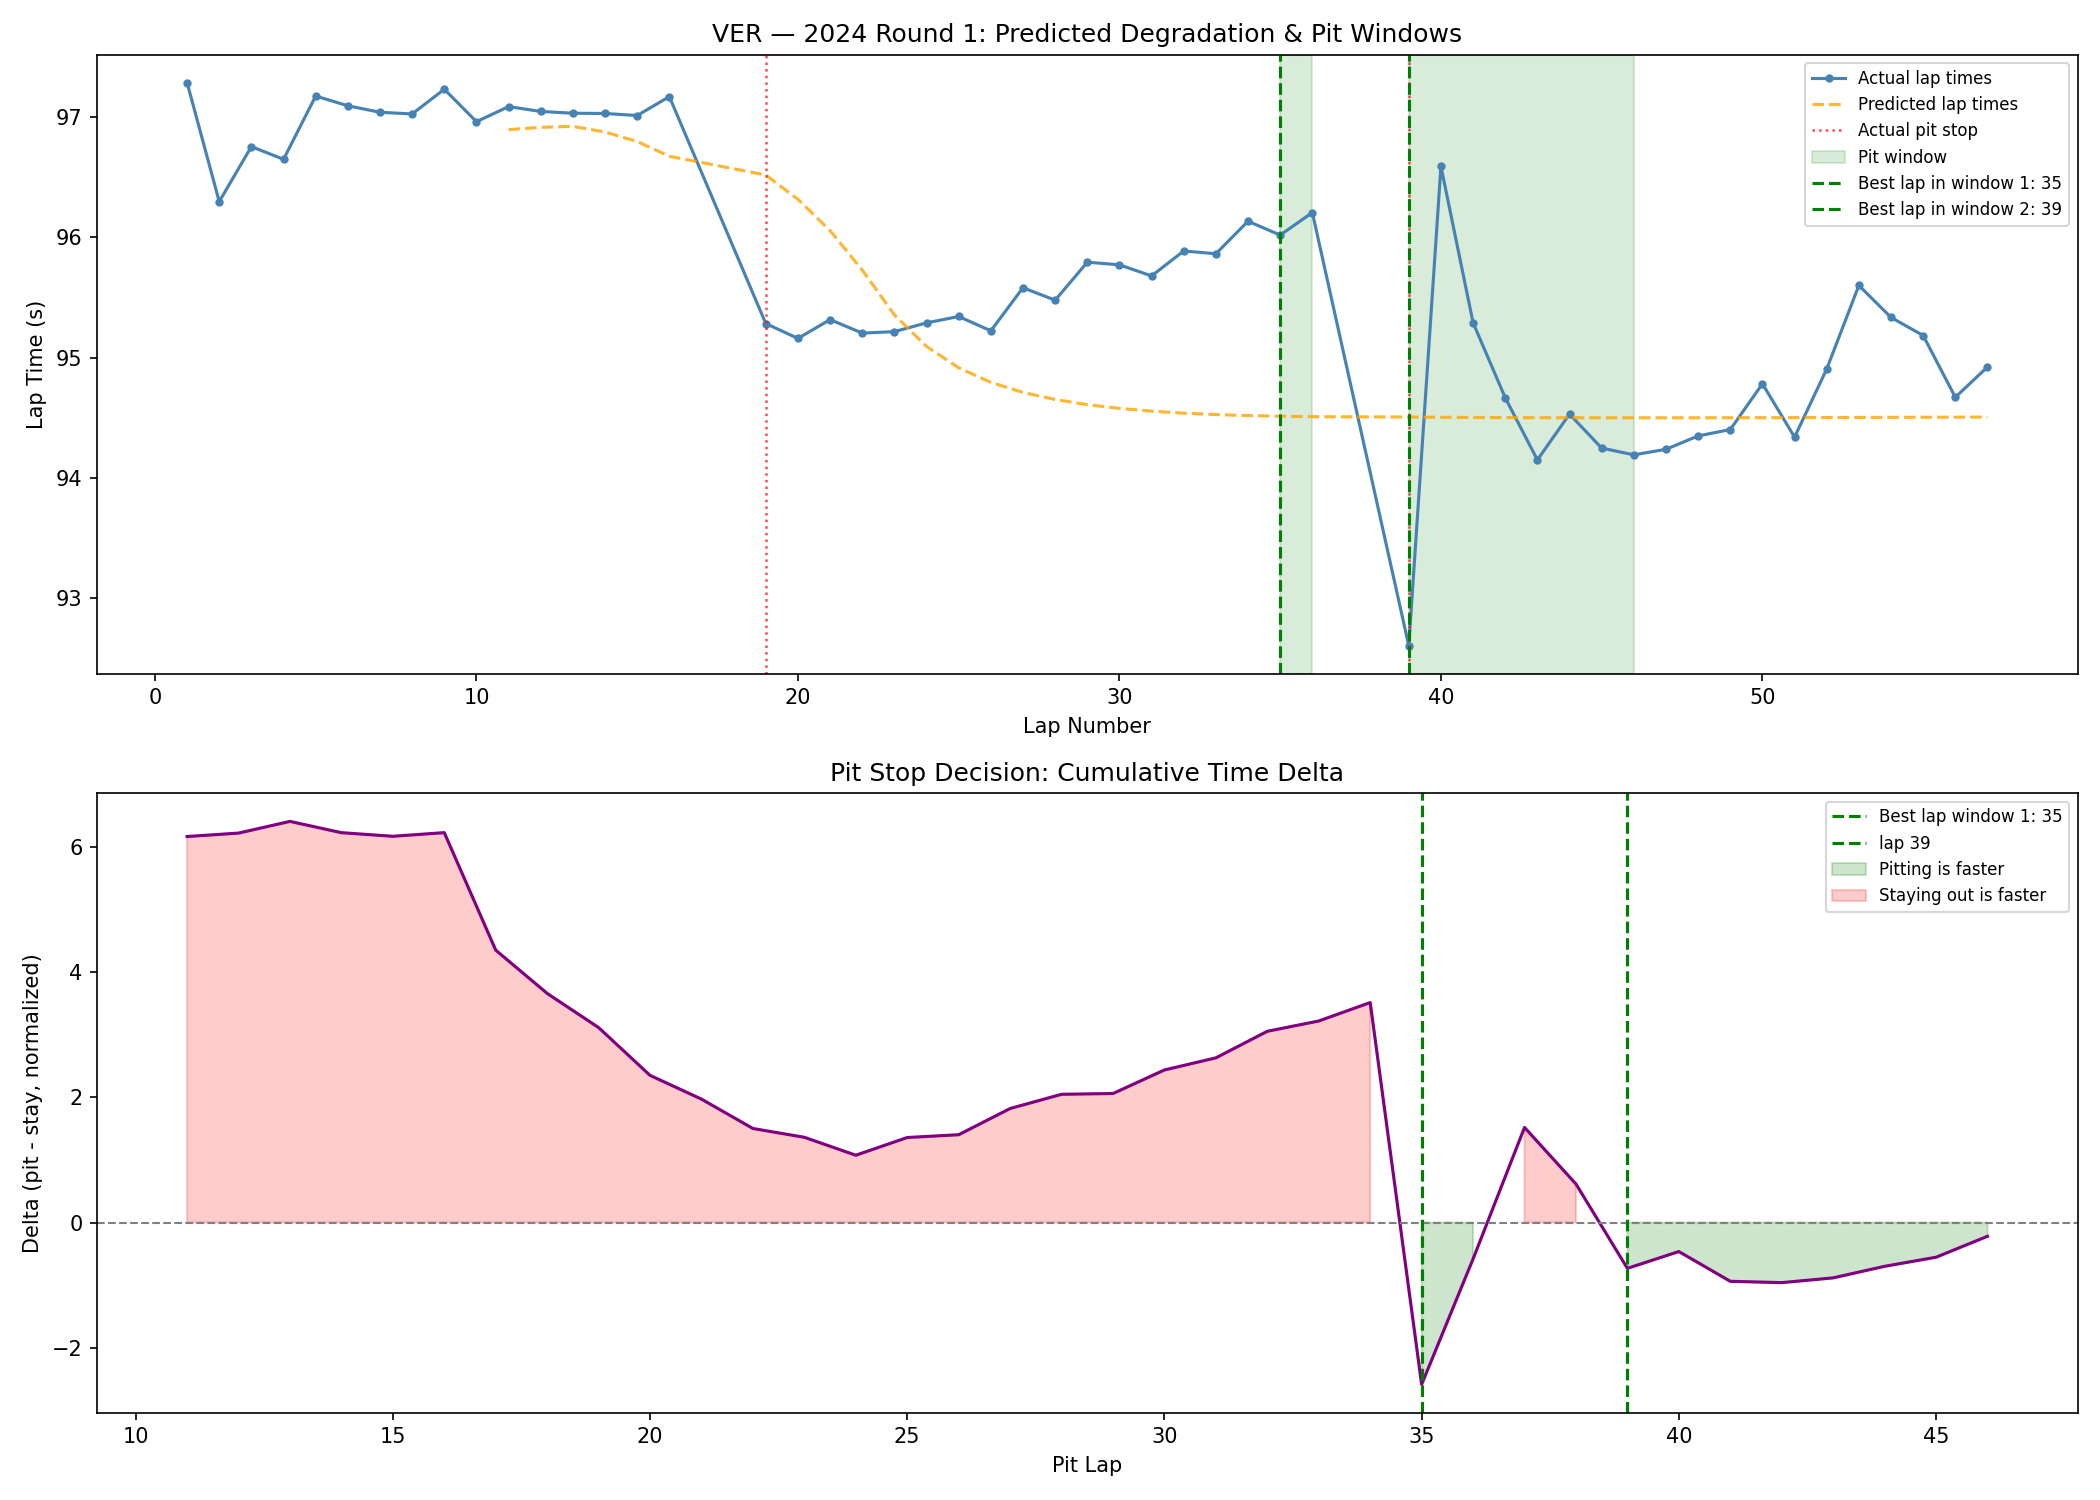
\includegraphics[width=\linewidth]{../results/strategy_VER_2024_r1.png}
    \caption{VER, Round 1 (Bahrain): correct prediction. Predicted pit window (green) brackets the actual stop at lap~38.}
    \label{fig:strat_ver}
\end{subfigure}
\hfill
\begin{subfigure}[t]{0.49\textwidth}
    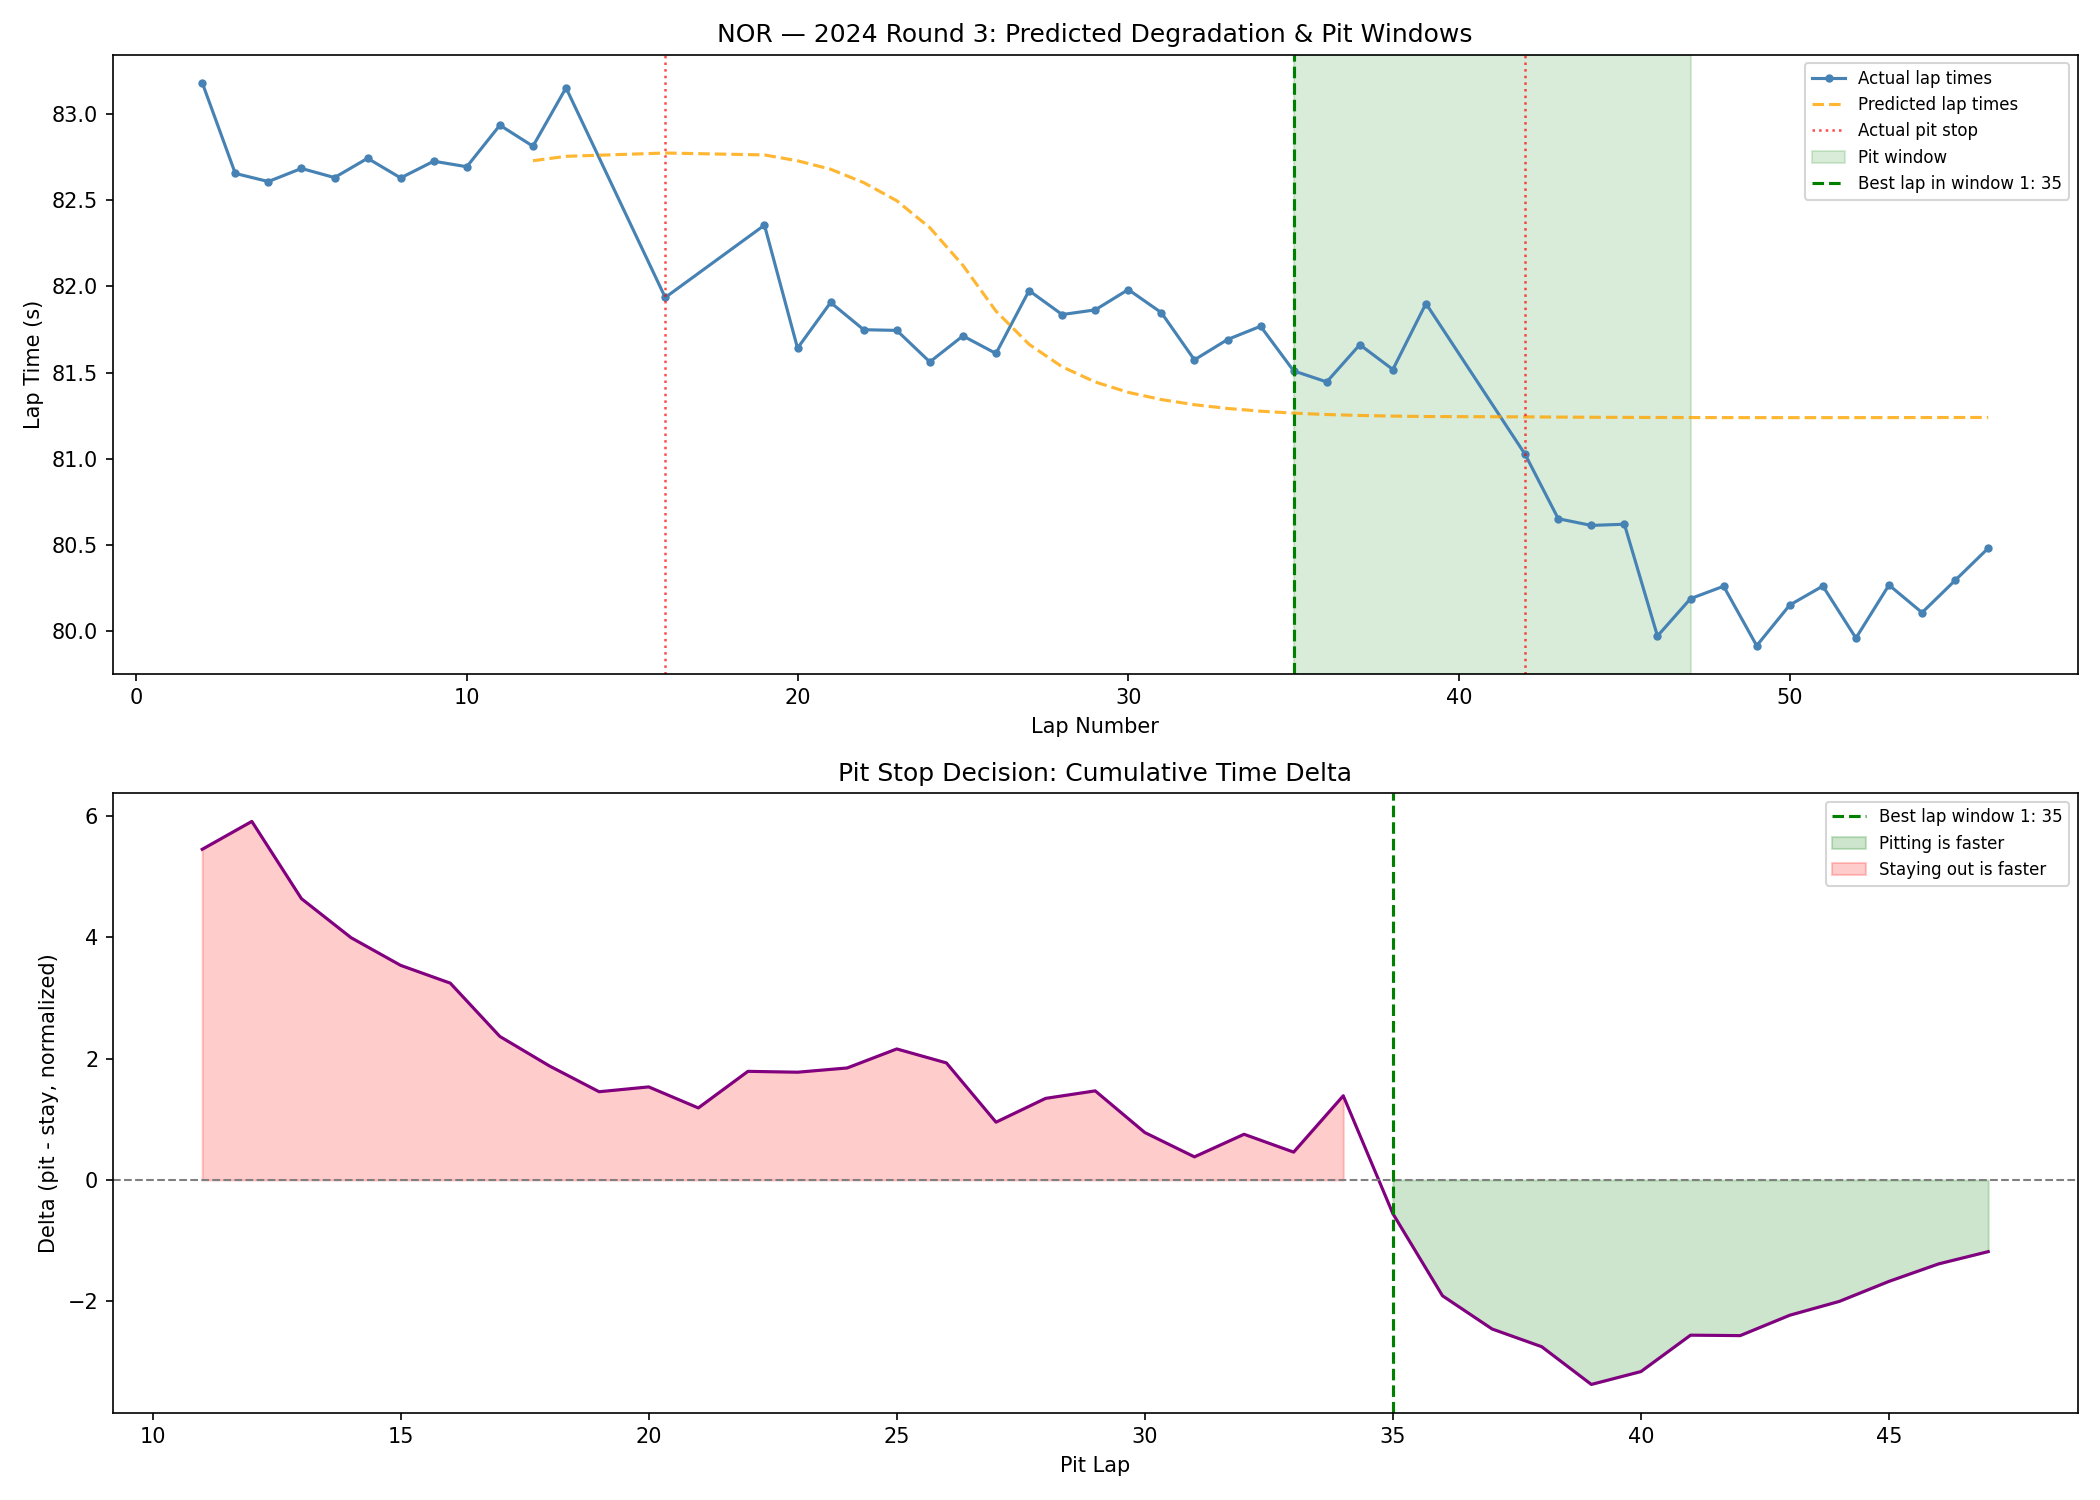
\includegraphics[width=\linewidth]{../results/strategy_NOR_2024_r3.png}
    \caption{NOR, Round 3 (Australia): miss. Actual stop on lap~13 was a tactical undercut; model predicted degradation-driven window at lap~35+.}
\label{fig:strat_nor}
\end{subfigure}
\caption{Representative strategy predictions. Top panel: actual vs.\ predicted lap times and predicted pit window. Bottom panel: cumulative time delta (positive = staying out is faster, negative = pitting is faster).}
\label{fig:strategy_examples}
\end{figure} 

\subsection{Analysis}\label{sec:analysis}

\subsubsection{GRU Dominates LSTM Variants}

The GRU outperformed all LSTM variants in every experimental configuration (Table~\ref{tab:architectures}, Figures~\ref{fig:training_curves}--\ref{fig:mae_comparison}). The margin is large: the GRU achieved a 38--40\% MAE improvement over the baseline, while the best-case LSTM only achieved 4--31\%.
Two factors explain this:

\textit{Parameter efficiency}: GRU has 39{,}425 parameters vs.\ 52{,}545 for LSTM (a 25\% reduction), lowering overfitting risk on a 28,000-sample training set. The consistent performance of high-dropout LSTM (+31.5\%) confirms that overfitting,not capacity, is the binding constraint.

\textit{Short sequence suitability}: With a 10-lap window, the cell state memory advantage of LSTM is irrelevant. Degradation within a 10-lap stint is approximately monotonic; complex long-range dependencies are absent. GRU's simpler update mechanism is well-matched to this structure.

\subsubsection{Attention Fails at Short Sequences}

LSTM with additive attention performed worst of all variants ($-22.5\%$ vs.\ baseline). With only 10 timesteps, the variation across hidden states is too small for the attention layer to learn a discriminative weighting; weights collapse toward uniform, and the additional non-linearity introduces noise. This is consistent with prior work showing attention benefits sequences of 20+ timesteps~\cite{bahdanau2015}.

\subsubsection{Delta Target is the Key Representation}

Switching the training target from absolute lap time to lap-to-lap delta ($\Delta t$) roughly doubled strategy accuracy (9.5\% $\to$ 19.0\%) on the original 42-evaluation pre-Phase-1 subset, without changing the model architecture. The 9.5\% baseline is the absolute-lap-time GRU result reported in Table~\ref{tab:decoupled} (Run 2 GRU); 19.0\% is the same architecture retrained on the delta target before any of the strategy-level phases in Table~\ref{tab:strategy} were applied. The improvement is conceptually clean since absolute lap time prediction forces the model to jointly explain baseline circuit pace and the marginal degradation signal, which are entangled in the normalized feature space. The delta formulation isolates the degradation rate as the sole target, which is what the strategy simulator actually needs.

Figure~\ref{fig:predictions} shows GRU predictions against held-out 2024 lap time sequences. The time series panel (top) shows the model tracking the degradation slope within each stint, including step changes at pit stops. The scatter plot (bottom) reveals a slight underprediction bias at high normalized lap times---corresponding to heavily degraded tires late in stints---which is where the pit crossover signal is most critical.

\begin{figure}[htbp]
\centering
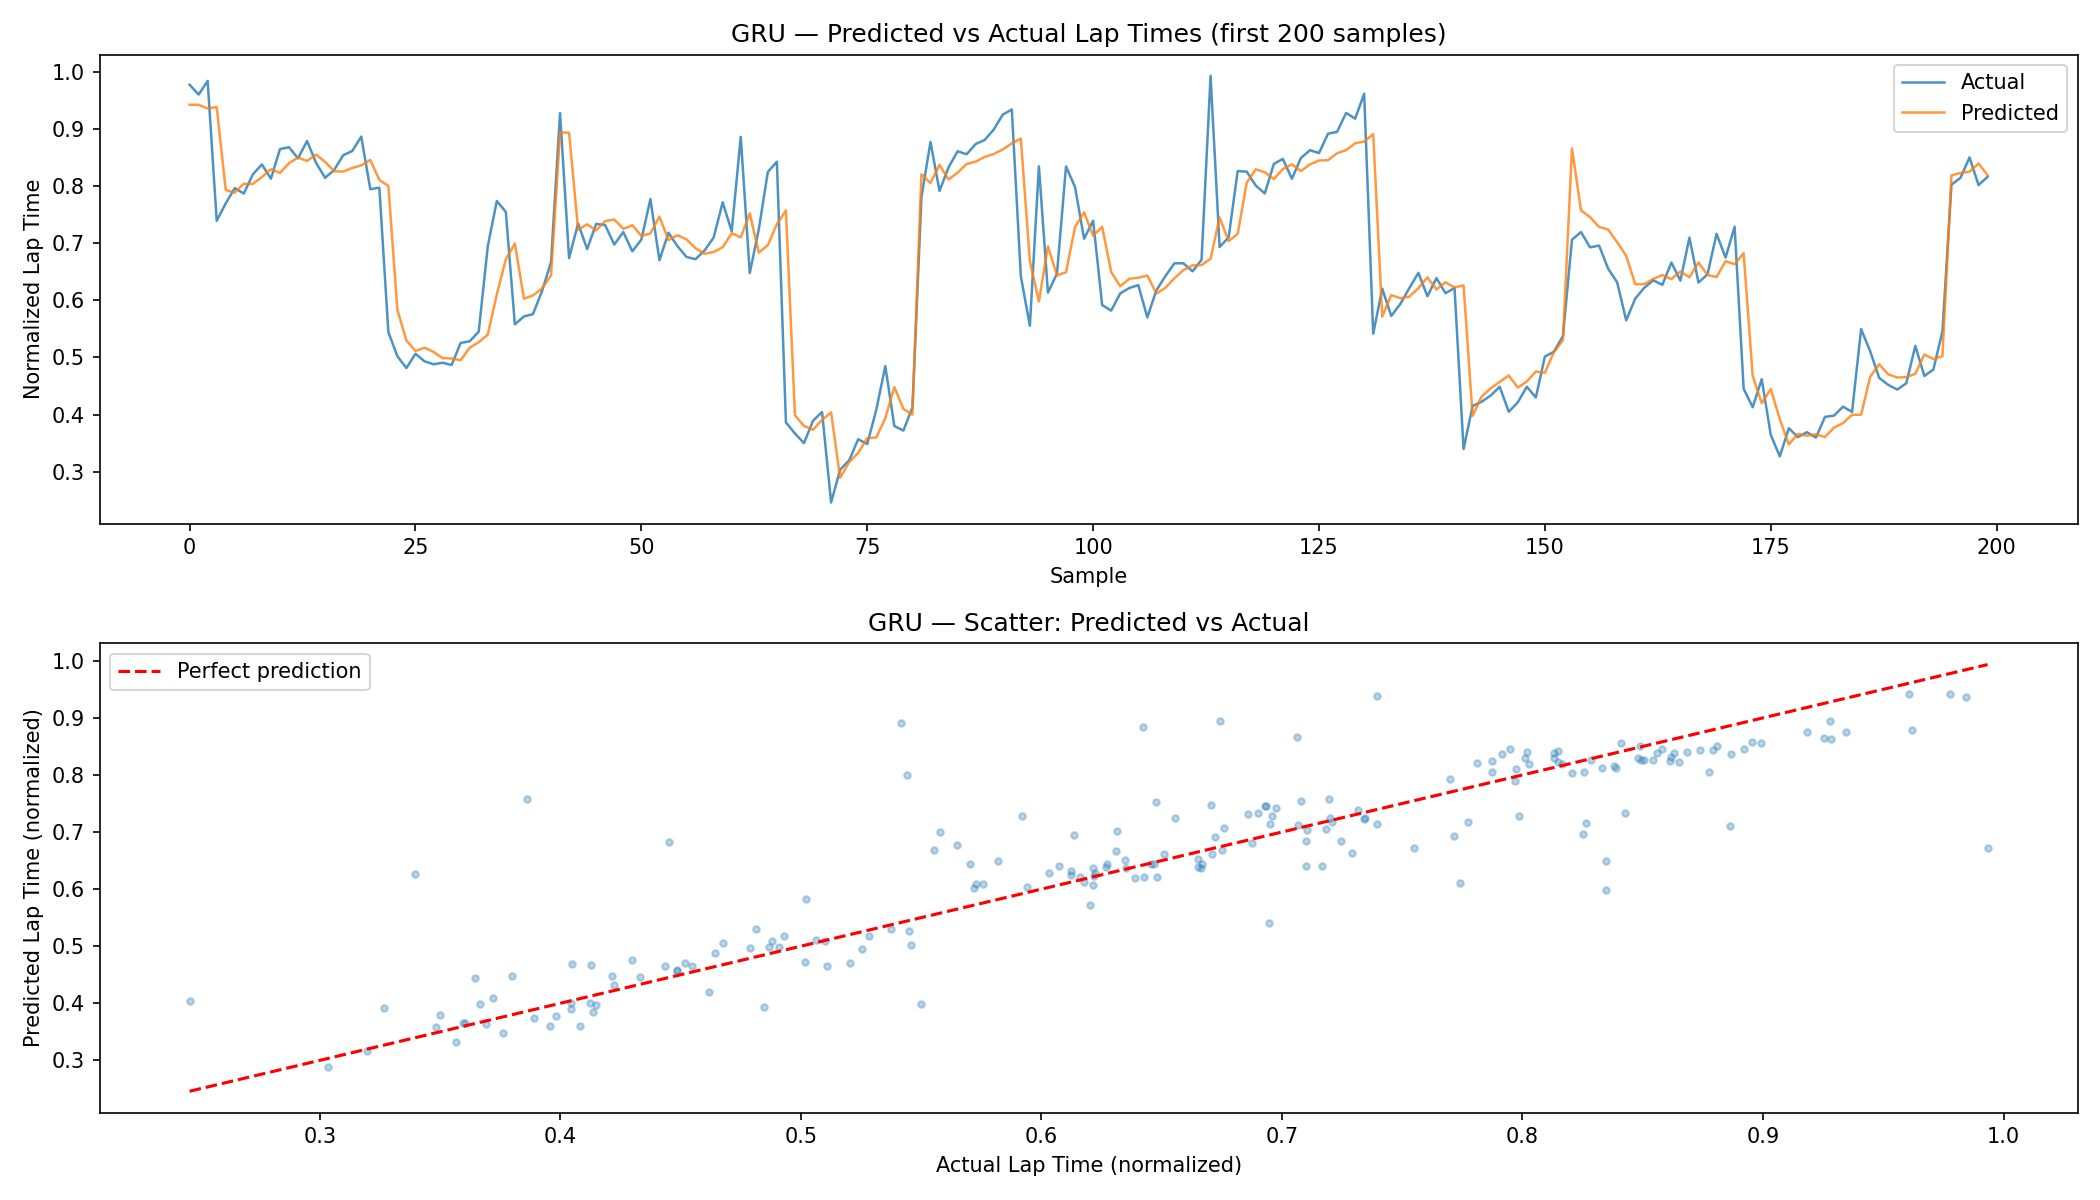
\includegraphics[width=\textwidth]{../results/predictions_gru.png}
\caption{GRU predictions on held-out 2024 sequences (first 200 samples). Top: predicted vs.\ actual lap time over time, showing accurate tracking of within-stint degradation slopes. Bottom: scatter of predicted vs.\ actual; the slight underprediction at high lap times indicates the model conservatively underestimates late-stint degradation.}
\label{fig:predictions}
\end{figure}

\FloatBarrier
\subsubsection{MAE and Strategy Accuracy Are Decoupled}

A striking pattern across three separate experiments is that lower test MAE does not imply higher strategy accuracy (Table~\ref{tab:decoupled}). Run 3 achieves the best MAE improvement (+40\%) but produces 0\% strategy accuracy. Run 6 (which adds the globally-normalized \texttt{TrackTemp\_global} feature alongside the existing per-race \texttt{TrackTemp}, giving the model both a circuit-relative and an absolute temperature signal) achieves better MAE than the best strategy-level configuration but yields only 2.4\% strategy accuracy.

\begin{table}[ht]
\centering
\caption{MAE vs.\ Strategy Accuracy Divergence}
\label{tab:decoupled}
\begin{tabular}{llrr}
\toprule
Configuration & Change & MAE Improvement & Strategy Accuracy \\
\midrule
Run 2 GRU & Baseline GRU & +38.5\% & 9.5\% \\
Run 3 GRU & SC filtering & +40.0\% & 0\% \\
Run 6 GRU & Global TrackTemp & +41.8\% & 2.4\% \\
Phase 2 compound GRU & Compound split & --- & \textbf{61.9\%} \\
\bottomrule
\end{tabular}
\end{table}

This divergence occurs because MAE measures accuracy on the test lap time distribution, while strategy accuracy measures timing quality on a different task: detecting the crossover point where pitting becomes net beneficial. A model that explains circuit-level temperature signals well (Run 6) may have lower MAE, but predict degradation slopes that are biased by those irrelevant signals, leading to systematically wrong pit timing.

\FloatBarrier
\subsubsection{Compound-Specific Models Are the Key Breakthrough}

The single largest accuracy improvement is achieved in Phase 2 by splitting training by tire compound ($+26.2$ percentage points over Phase 1). A shared GRU must average degradation behavior across SOFT, MEDIUM, and HARD compounds, whose degradation rates differ by a factor of 2--3. A compound-specific model sees only the degradation behavior relevant to the current tire, producing sharper predictions near the pit window crossover.

\FloatBarrier
\subsubsection{Negative Experiments}

Two experiments were reverted after causing regression:

\textit{Phase 3 --- Minimum first-pit constraint}: A hard lower bound of $\max(15, 0.2 \times L_\text{total})$ laps was imposed on the first pit recommendation to eliminate spurious early-pit predictions. This yielded 59.5\% (vs.\ 61.9\%), as it broke two races where early pits (laps 13--15) were strategically correct (Japan undercut, China sprint). A fixed minimum is too blunt without circuit-specific context.

\textit{Phase 4 --- Longer sequence (seq=15)}: Increasing the window from 10 to 15 laps reduced training sequences by 15\% (fewer stints long enough to yield 15-lap windows) and shifted the model's first-prediction opportunity later in each stint, producing an accuracy of 50.0\%.

\FloatBarrier
\subsubsection{Per-Driver Spread Reveals Identity Bottleneck}

The 30 percent spread in Table~\ref{tab:drivers} (HAM 40\% $\to$ RUS 70\%) cannot be explained by team effects---same-team pairs diverge significantly (HAM 40\% vs.\ RUS 70\% on Mercedes; LEC 45\% vs.\ SAI 60\% on Ferrari). This points to driver-specific stint patterns that the current model cannot capture. Russell ran notably more conservative stint strategies in 2024 (later first pits, consistent MEDIUM stints) that align well with the model's predictions; Hamilton's more aggressive tire management and frequent off-sequence stops are harder to predict.

The NOR miss in Figure~\ref{fig:strat_nor} is emblematic of this class of failure. The model correctly identifies when degradation would warrant a stop, but cannot anticipate that the team will sacrifice lap time to execute a tactical undercut instead. The model has no driver or team identity feature. Adding driver one-hot encoding or team-level embeddings would be the most impactful next step.
